% Provenance (never printed): cycle 4 SVT, "La planete Terre": volcanic
% activity, its products and its link with plate boundaries; natural hazards
% and their monitoring; see sources/book1/PROVENANCE.md. Book 1, grade 7,
% chapter 2.
% Vocabulary guard: "magma" first allowed here; "sediment" not before g7.4;
% "subduction zone" is never a term here (gloss: "where one plate sinks under
% another"); "hotspot track" is Book 2's; lahars are called mudflows.
\chapter{Os vulcões}\label{ch:g7:volcanoes}

Em 17~de~maio~de~1980, um geólogo estava num espigão a dez quilômetros do
monte Santa Helena, no noroeste dos Estados Unidos, e tirou a fotografia da
esquerda, abaixo: um cone liso e nevado, uma das \omterm{def:g1:landscapes-around-us:landform}{montanhas} mais elegantes
do país. Havia dois meses que a \omterm{def:g1:landscapes-around-us:landform}{montanha} tremia, e a sua face norte estava
inchando para fora como um balão. Na manhã seguinte, às 8h32, um pequeno
\omterm{def:g4:volcanoes-earthquakes-first-look:earthquake}{terremoto} a sacudiu. Toda a face inchada deslizou, e o \omterm{def:g4:volcanoes-earthquakes-first-look:volcano}{vulcão} explodiu de
lado. Quando o mesmo espigão pôde ser fotografado de novo, em setembro, a
\omterm{def:g1:landscapes-around-us:landform}{montanha} estava como na fotografia da direita.

\begin{omfigure}
\begin{minipage}[b]{0.495\linewidth}\centering
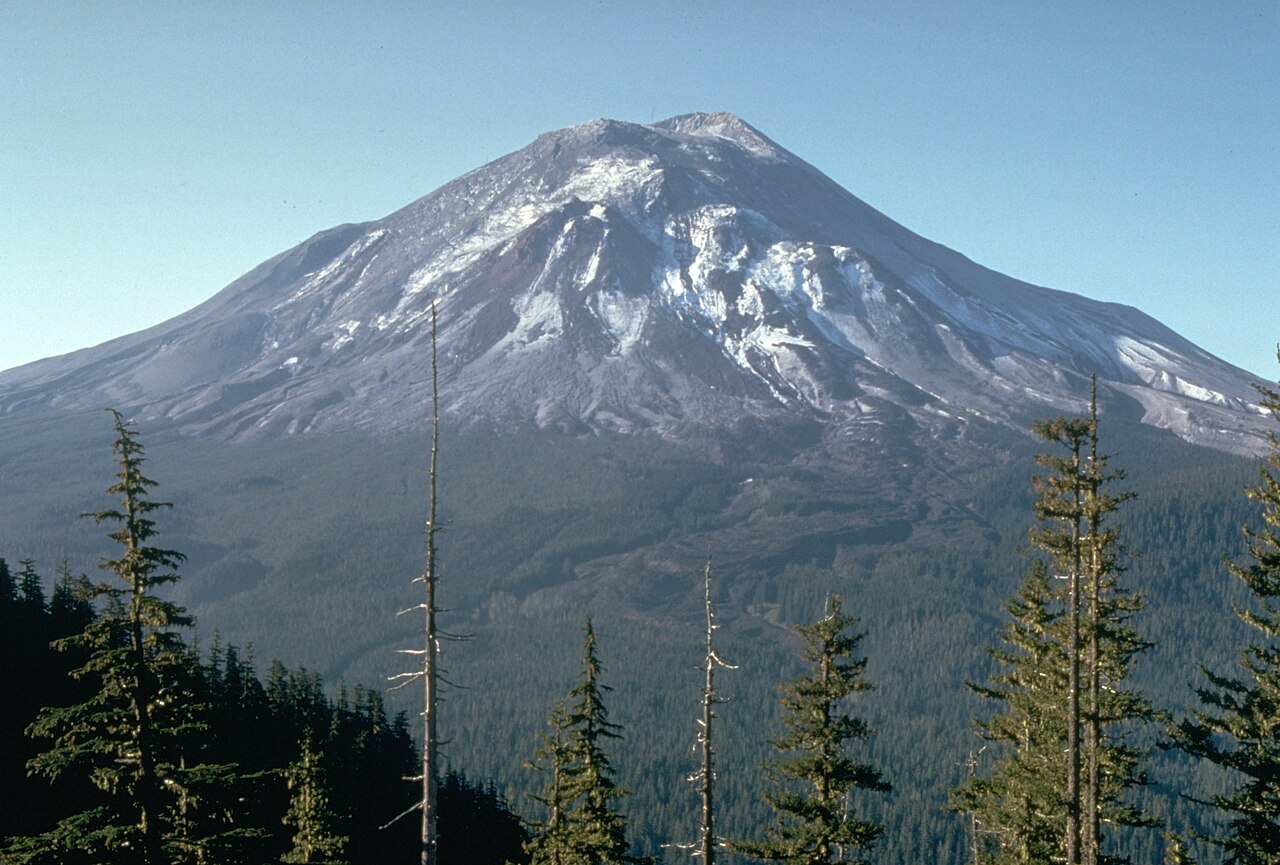
\includegraphics[width=\linewidth]{images/book1/g7-msh-before.jpg}

{\small 17 de maio de 1980, a véspera.}
\end{minipage}\hfill
\begin{minipage}[b]{0.495\linewidth}\centering
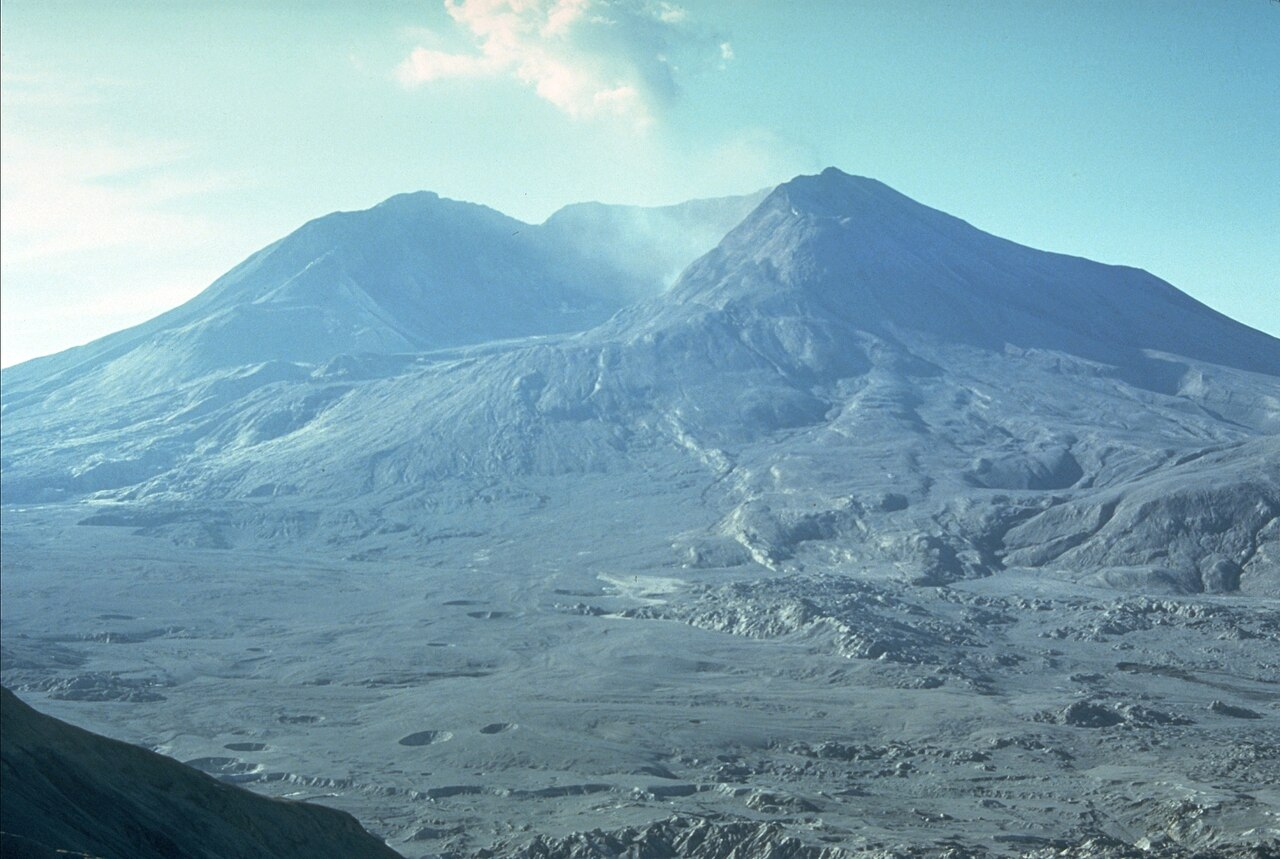
\includegraphics[width=\linewidth]{images/book1/g7-msh-after.jpg}

{\small 10 de setembro de 1980.}
\end{minipage}

{\small O monte Santa Helena visto de Johnston Ridge, antes e depois da
\omterm{def:g4:volcanoes-earthquakes-first-look:eruption}{erupção} de 18~de~maio~de~1980. O cume e toda a face norte desapareceram;
uma \omterm{def:g7:volcanoes:vent}{cratera} aberta para o norte tomou o seu lugar. Fotografias: Harry
Glicken, U.S. Geological Survey (domínio público, via Wikimedia Commons).}
% ledger: commons:msh-before, commons:msh-after, usgs:msh-lead-up, usgs:msh-may18
\label{fig:g7:volcanoes:st-helens}
\end{omfigure}

Neste capítulo, abrimos um \omterm{def:g4:volcanoes-earthquakes-first-look:volcano}{vulcão} para ver o que provoca uma \omterm{def:g4:volcanoes-earthquakes-first-look:eruption}{erupção};
descobrimos por que alguns \omterm{def:g4:volcanoes-earthquakes-first-look:volcano}{vulcões} derramam \omterm{def:g1:landscapes-around-us:water}{rios} tranquilos de \omterm{def:g4:volcanoes-earthquakes-first-look:eruption}{lava} enquanto
outros explodem em pedaços; e olhamos de novo o \omterm{def:g3:continents-and-oceans:world-map}{mapa-múndi}, para ver onde
ficam os \omterm{def:g4:volcanoes-earthquakes-first-look:volcano}{vulcões} e por quê.

\begin{recall}
Um \emph{\omterm{def:g4:volcanoes-earthquakes-first-look:volcano}{vulcão}} é um lugar onde a \omterm{def:g3:stones-pebbles-sand:rock}{rocha} derretida do interior profundo da
Terra sai na superfície, e o morro ou a \omterm{def:g1:landscapes-around-us:landform}{montanha} que ela constrói ali.
Durante uma \emph{\omterm{def:g4:volcanoes-earthquakes-first-look:eruption}{erupção}}, ele lança \omterm{def:g4:volcanoes-earthquakes-first-look:eruption}{lava}, cinzas e gases
(\cref{ch:g4:volcanoes-earthquakes-first-look}). Embaixo da \omterm{def:g6:inside-the-earth:layers}{crosta}, o \omterm{def:g6:inside-the-earth:layers}{manto}
é feito de \omterm{def:g3:stones-pebbles-sand:rock}{rocha} quente que é sólida, embora possa se deslocar muito
devagar (\cref{ch:g6:inside-the-earth}). O basalto e o granito são \omterm{def:g6:rocks-and-minerals:rock-families}{rochas
ígneas}: eles se formam quando a \omterm{def:g3:stones-pebbles-sand:rock}{rocha} derretida esfria e endurece
(\cref{ch:g6:rocks-and-minerals}). A casca externa da Terra está partida
em placas que se movem alguns centímetros por ano; as suas bordas são os
\omterm{def:g7:plate-tectonics:plate-boundary}{limites de placas} (\cref{ch:g7:plate-tectonics}).
\end{recall}

\section{Dentro de um vulcão}

O \omterm{def:g6:inside-the-earth:layers}{manto} é sólido. Mesmo assim, em alguns lugares, bem fundo embaixo da
superfície, uma pequena parte da \omterm{def:g3:stones-pebbles-sand:rock}{rocha} derrete. A \omterm{def:g3:stones-pebbles-sand:rock}{rocha} derretida é mais
leve que a \omterm{def:g3:stones-pebbles-sand:rock}{rocha} sólida em volta dela, então ela sobe devagar, se
espremendo por rachaduras, como uma gota de óleo que sobe na água.
% ledger: usgs:hawaii-hotspot (magma lighter than the surrounding rock, rises)

\begin{definition}[Magma]\label{def:g7:volcanoes:magma}
O \emph{magma}\index{magma} é a \omterm{def:g3:stones-pebbles-sand:rock}{rocha} derretida embaixo da terra. É um
líquido quente que também pode levar cristais e, dissolvidos nele, gases
como o vapor de água e o gás carbônico. O magma que sai na superfície se
chama \omterm{def:g4:volcanoes-earthquakes-first-look:eruption}{lava}; ao sair, ele perde a maior parte do seu gás.
\end{definition}

O \omterm{def:g7:volcanoes:magma}{magma} que sobe muitas vezes para no caminho, a alguns quilômetros
abaixo da superfície, onde se acumula num grande bolsão. Ali ele espera,
às vezes durante séculos, até que uma \omterm{def:g4:volcanoes-earthquakes-first-look:eruption}{erupção} esvazie uma parte dele.

\begin{definition}[Câmara magmática]\label{def:g7:volcanoes:magma-chamber}
Uma \emph{câmara magmática}\index{camara magmatica@câmara magmática} é um grande espaço
nas \omterm{def:g3:stones-pebbles-sand:rock}{rochas} embaixo de um \omterm{def:g4:volcanoes-earthquakes-first-look:volcano}{vulcão}, a alguns quilômetros de profundidade, onde
o \omterm{def:g7:volcanoes:magma}{magma} se acumula antes de uma \omterm{def:g4:volcanoes-earthquakes-first-look:eruption}{erupção}.
\end{definition}

\begin{definition}[Boca e cratera]\label{def:g7:volcanoes:vent}
Uma \emph{boca}\index{boca (de um vulcao)@boca (de um vulcão)} é uma abertura na superfície por onde saem o
\omterm{def:g7:volcanoes:magma}{magma}, os gases e as cinzas. Uma \emph{cratera}\index{cratera} é a depressão em
forma de tigela em volta de uma boca, em geral no alto do \omterm{def:g4:volcanoes-earthquakes-first-look:volcano}{vulcão}.
\end{definition}

\begin{omfigure}
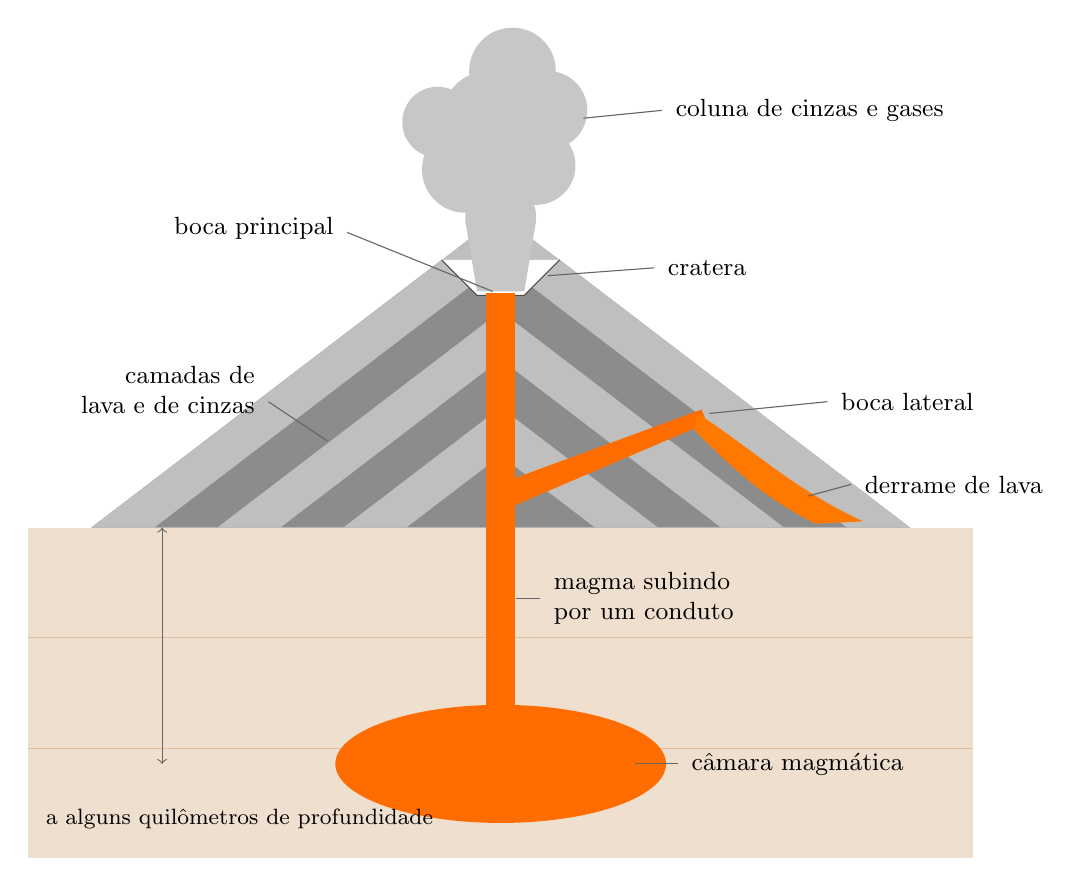
\begin{tikzpicture}[font=\small, x=1cm, y=1cm]
  % rocks below the volcano
  \fill[brown!25] (-6,-4.2) rectangle (6,0);
  \draw[brown!50] (-6,-1.4) -- (6,-1.4) (-6,-2.8) -- (6,-2.8);
  % the cone, built of layers of lava (dark) and ash (light)
  \fill[black!45] (-5.2,0) -- (-0.75,3.4) -- (0.75,3.4) -- (5.2,0) -- cycle;
    % layers dipping outwards, parallel to the flanks (slope 3.4/4.45)
  \foreach \k/\c in {0/black!25, 2/black!25, 4/black!25} {
    \pgfmathsetmacro{\xa}{-5.2+0.8*\k}\pgfmathsetmacro{\xb}{-5.2+0.8*(\k+1)}
    \pgfmathsetmacro{\ya}{(-0.18-\xa)*3.4/4.45}\pgfmathsetmacro{\yb}{(-0.18-\xb)*3.4/4.45}
    \fill[\c] (\xa,0) -- (-0.18,\ya) -- (-0.18,\yb) -- (\xb,0) -- cycle;
    \fill[\c] (-\xa,0) -- (0.18,\ya) -- (0.18,\yb) -- (-\xb,0) -- cycle;
  }
  % the crater at the top
  \fill[white] (-0.75,3.4) -- (-0.3,2.95) -- (0.3,2.95) -- (0.75,3.4) -- cycle;
  \draw[black!70] (-0.75,3.4) -- (-0.3,2.95) -- (0.3,2.95) -- (0.75,3.4);
  % magma chamber and the pipe up to the vent
  \fill[orange!85!red] (0,-3.0) ellipse (2.1 and 0.75);
  \fill[orange!85!red] (-0.18,-2.4) rectangle (0.18,2.98);
  % a side branch to a small side vent
  \fill[orange!85!red] (0.1,0.6) -- (2.55,1.5) -- (2.62,1.33) -- (0.1,0.25) -- cycle;
  % lava flow down the right flank, from the side vent
  \fill[orange!95!red] (2.5,1.45) .. controls (3.2,1.0) and (3.7,0.5) .. (4.6,0.08)
    -- (4.0,0.05) .. controls (3.3,0.4) and (2.9,0.8) .. (2.45,1.25) -- cycle;
  % ash column and gas
    \fill[black!22] (-0.3,3.0) -- (0.3,3.0) -- (0.45,3.9) -- (-0.45,3.9) -- cycle;
  \foreach \x/\y/\r in {0/3.95/0.45, -0.45/4.55/0.55, 0.45/4.6/0.5, -0.15/5.2/0.6,
                        0.6/5.3/0.5, -0.8/5.15/0.45, 0.15/5.8/0.55}
    \fill[black!22] (\x,\y) circle (\r);
  % labels
  \node[anchor=west] at (2.1,5.3) {coluna de cinzas e gases};
  \draw[black!60] (2.05,5.3) -- (1.05,5.2);
  \node[anchor=west] at (2.0,3.3) {cratera};
  \draw[black!60] (1.95,3.3) -- (0.6,3.2);
  \node[anchor=east] at (-2.0,3.8) {boca principal};
  \draw[black!60] (-1.95,3.75) -- (-0.1,3.0);
  \node[anchor=west] at (4.2,1.6) {boca lateral};
  \draw[black!60] (4.15,1.6) -- (2.65,1.45);
  \node[anchor=west] at (4.5,0.55) {derrame de lava};
  \draw[black!60] (4.45,0.55) -- (3.9,0.4);
  \node[anchor=east, align=right] at (-3.0,1.75) {camadas de\\lava e de cinzas};
  \draw[black!60] (-2.95,1.6) -- (-2.2,1.1);
  \node[anchor=west, align=left] at (0.55,-0.9) {magma subindo\\por um conduto};
  \draw[black!60] (0.5,-0.9) -- (0.2,-0.9);
  \node[anchor=west] at (2.3,-3.0) {câmara magmática};
  \draw[black!60] (2.25,-3.0) -- (1.7,-3.0);
  \node[anchor=west, align=left, font=\footnotesize] at (-5.9,-3.7) {a alguns quilômetros de profundidade};
  \draw[black!60, <->] (-4.3,0) -- (-4.3,-3.0);
\end{tikzpicture}

{\small Um \omterm{def:g4:volcanoes-earthquakes-first-look:volcano}{vulcão} aberto (um desenho, fora de escala). O \omterm{def:g7:volcanoes:magma}{magma} se acumula
na \omterm{def:g7:volcanoes:magma-chamber}{câmara magmática} e sobe por um conduto até a \omterm{def:g7:volcanoes:vent}{boca} principal, no fundo
da \omterm{def:g7:volcanoes:vent}{cratera}; um ramo chega a uma \omterm{def:g7:volcanoes:vent}{boca} lateral, na encosta. Cada \omterm{def:g4:volcanoes-earthquakes-first-look:eruption}{erupção}
acrescenta uma camada de \omterm{def:g4:volcanoes-earthquakes-first-look:eruption}{lava} ou de cinzas ao cone.}
\label{fig:g7:volcanoes:cutaway}
\end{omfigure}

Então a mesma \omterm{def:g3:stones-pebbles-sand:rock}{rocha} derretida tem dois nomes. Embaixo da terra, ela é
\emph{\omterm{def:g7:volcanoes:magma}{magma}}; depois de sair por uma \omterm{def:g7:volcanoes:vent}{boca}, ela é \emph{\omterm{def:g4:volcanoes-earthquakes-first-look:eruption}{lava}}. A diferença
não é só uma questão de palavras: o \omterm{def:g7:volcanoes:magma}{magma} ainda guarda o seu gás, enquanto
a \omterm{def:g4:volcanoes-earthquakes-first-look:eruption}{lava} perdeu a maior parte dele para o ar. Vamos ver que é esse gás que
decide o tipo de \omterm{def:g4:volcanoes-earthquakes-first-look:eruption}{erupção} de um \omterm{def:g4:volcanoes-earthquakes-first-look:volcano}{vulcão}.

Qual é a temperatura? Os cientistas do Observatório Vulcanológico do Havaí
medem a \omterm{def:g4:volcanoes-earthquakes-first-look:eruption}{lava} quando ela sai das \omterm{def:g7:volcanoes:vent}{bocas} do Kilauea, um dos \omterm{def:g4:volcanoes-earthquakes-first-look:volcano}{vulcões} do Havaí:
cerca de \qty{1170}{\degreeCelsius}. A \omterm{def:g3:stones-pebbles-sand:rock}{rocha} quente brilha, e a cor do
brilho depende da sua temperatura: câmeras especiais leem de longe a
temperatura de um derrame medindo as cores do seu brilho. Até o olho tem
uma ideia aproximada, como mostra a tabela.
% ledger: usgs:kilauea-temp, usgs:pyrometer

\begin{center}
\small
\begin{tabular}{|l|c|}
\hline
\textbf{cor da \omterm{def:g3:stones-pebbles-sand:rock}{rocha} incandescente} & \textbf{temperatura} \\
\hline
amarela & de cerca de 1000 a \qty{1200}{\degreeCelsius} \\
laranja & de cerca de 800 a \qty{1000}{\degreeCelsius} \\
vermelha & de cerca de 600 a \qty{800}{\degreeCelsius} \\
\hline
\end{tabular}
\end{center}
% ledger: usgs:kilauea-temp

\begin{remark}[Uma pele que esfria num segundo]\label{rem:g7:volcanoes:skin}
% ledger: usgs:kilauea-temp
Quando a \omterm{def:g4:volcanoes-earthquakes-first-look:eruption}{lava} encontra o ar, a sua superfície esfria centenas de graus por
segundo: uma pele escura se forma na hora sobre a \omterm{def:g3:stones-pebbles-sand:rock}{rocha} incandescente.
Embaixo da pele, a \omterm{def:g4:volcanoes-earthquakes-first-look:eruption}{lava} continua quente por muito tempo. No Havaí, a \omterm{def:g4:volcanoes-earthquakes-first-look:eruption}{lava}
já correu em túneis embaixo do seu próprio teto endurecido por
\qty{10}{km}, de uma \omterm{def:g7:volcanoes:vent}{boca} até o \omterm{def:g2:water-on-earth:ocean}{mar}, e ainda chegou à praia a cerca de
\qty{1140}{\degreeCelsius}: só cerca de 30~graus mais fria que na \omterm{def:g7:volcanoes:vent}{boca}.
\end{remark}

\begin{omfigure}
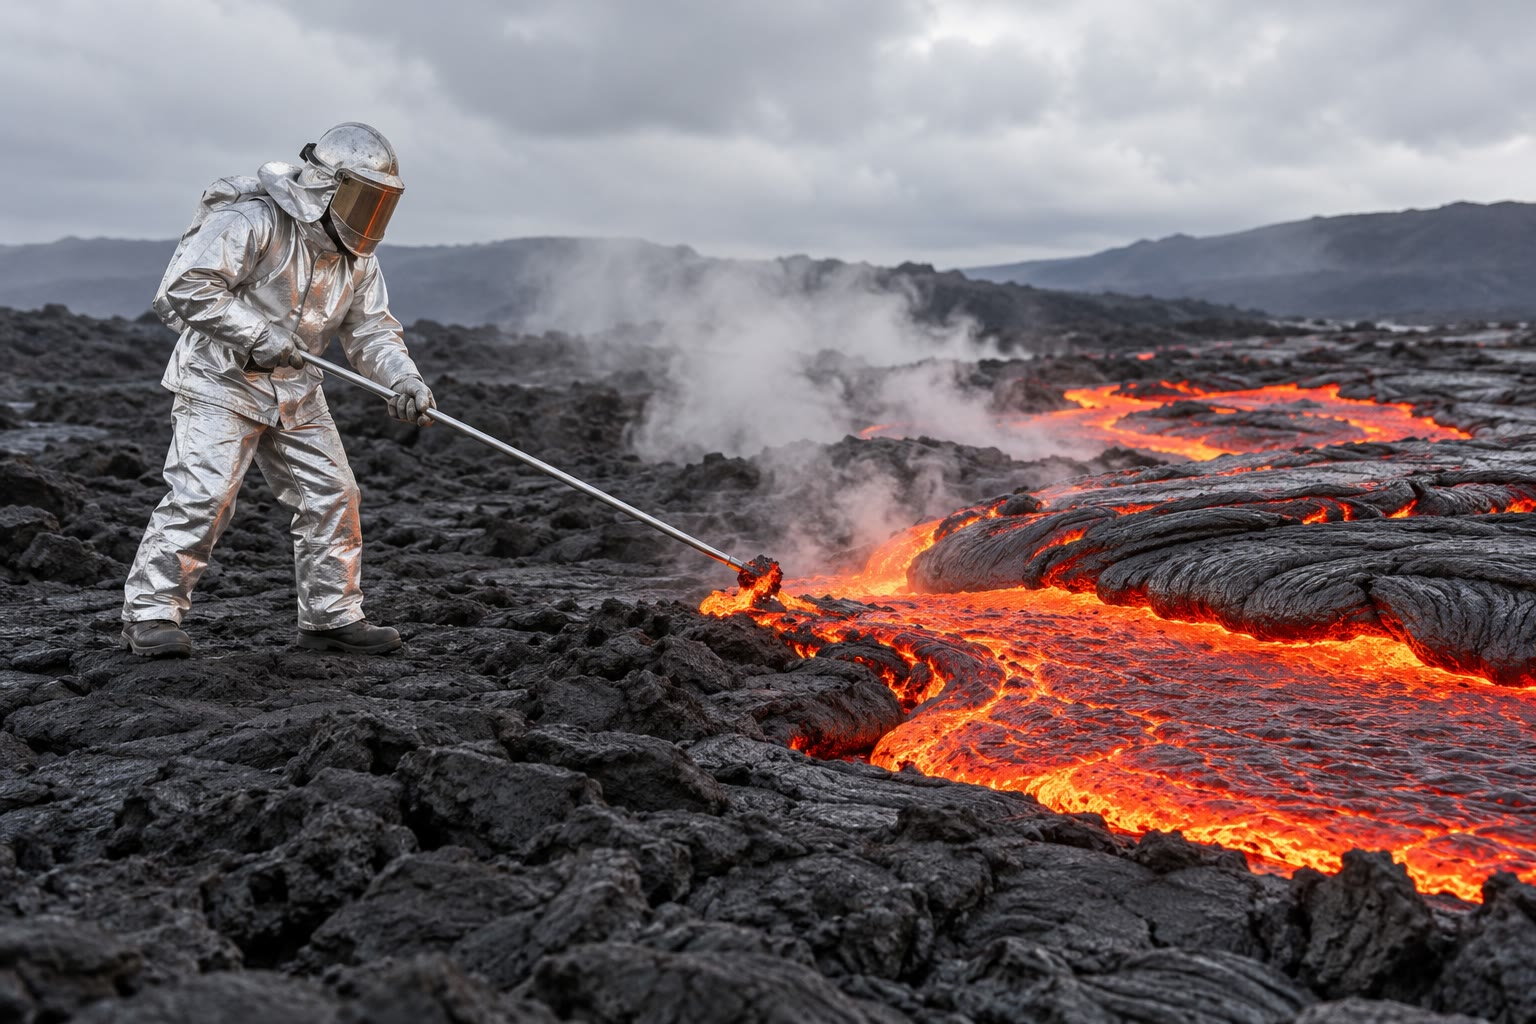
\includegraphics[width=0.6\linewidth]{images/book1/ai/g7-volcanologist.jpg}

{\small Uma vulcanóloga com uma roupa que reflete o calor recolhe uma
amostra de \omterm{def:g4:volcanoes-earthquakes-first-look:eruption}{lava} com uma longa vara de aço (ilustração de uma cena genérica
feita por IA). Só cientistas treinados, com esse tipo de equipamento,
chegam perto da \omterm{def:g4:volcanoes-earthquakes-first-look:eruption}{lava} que corre; todos os outros observam de onde as
autoridades permitem.}
\label{fig:g7:volcanoes:volcanologist}
\end{omfigure}

\section{Duas maneiras de entrar em erupção}

O monte Santa Helena explodiu em pedaços. Os \omterm{def:g4:volcanoes-earthquakes-first-look:volcano}{vulcões} do Havaí, ao
contrário, em geral derramam uma \omterm{def:g4:volcanoes-earthquakes-first-look:eruption}{lava} que corre encosta abaixo. Os
geólogos classificam as \omterm{def:g4:volcanoes-earthquakes-first-look:eruption}{erupções} em dois tipos.

\begin{definition}[Erupções efusivas e explosivas]\label{def:g7:volcanoes:eruption-types}
Numa \emph{erupção efusiva}\index{erupcao efusiva@erupção efusiva} o \omterm{def:g7:volcanoes:magma}{magma} sai tranquilamente
como \omterm{def:g4:volcanoes-earthquakes-first-look:eruption}{lava}, que corre para longe da \omterm{def:g7:volcanoes:vent}{boca}, às vezes por quilômetros, ou
jorra em fontes de gotas incandescentes. Numa \emph{erupção
explosiva}\index{erupcao explosiva@erupção explosiva} o \omterm{def:g7:volcanoes:magma}{magma} é despedaçado pelo seu próprio
gás: uma coluna de cinzas, de gases e de pedaços de \omterm{def:g3:stones-pebbles-sand:rock}{rocha} é lançada bem
alto no céu.
\end{definition}

\begin{omfigure}
\begin{minipage}[t]{0.49\linewidth}\centering
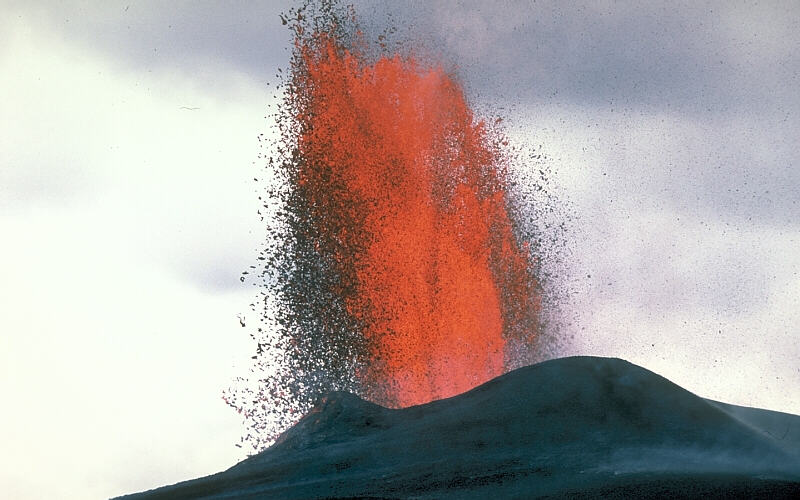
\includegraphics[height=4.5cm]{images/book1/g7-lava-fountain.jpg}

{\small Efusiva: uma fonte de lava no Kilauea, Havaí, 1983. Foto:
J.~D. Griggs, USGS.}
\end{minipage}\hfill
\begin{minipage}[t]{0.49\linewidth}\centering
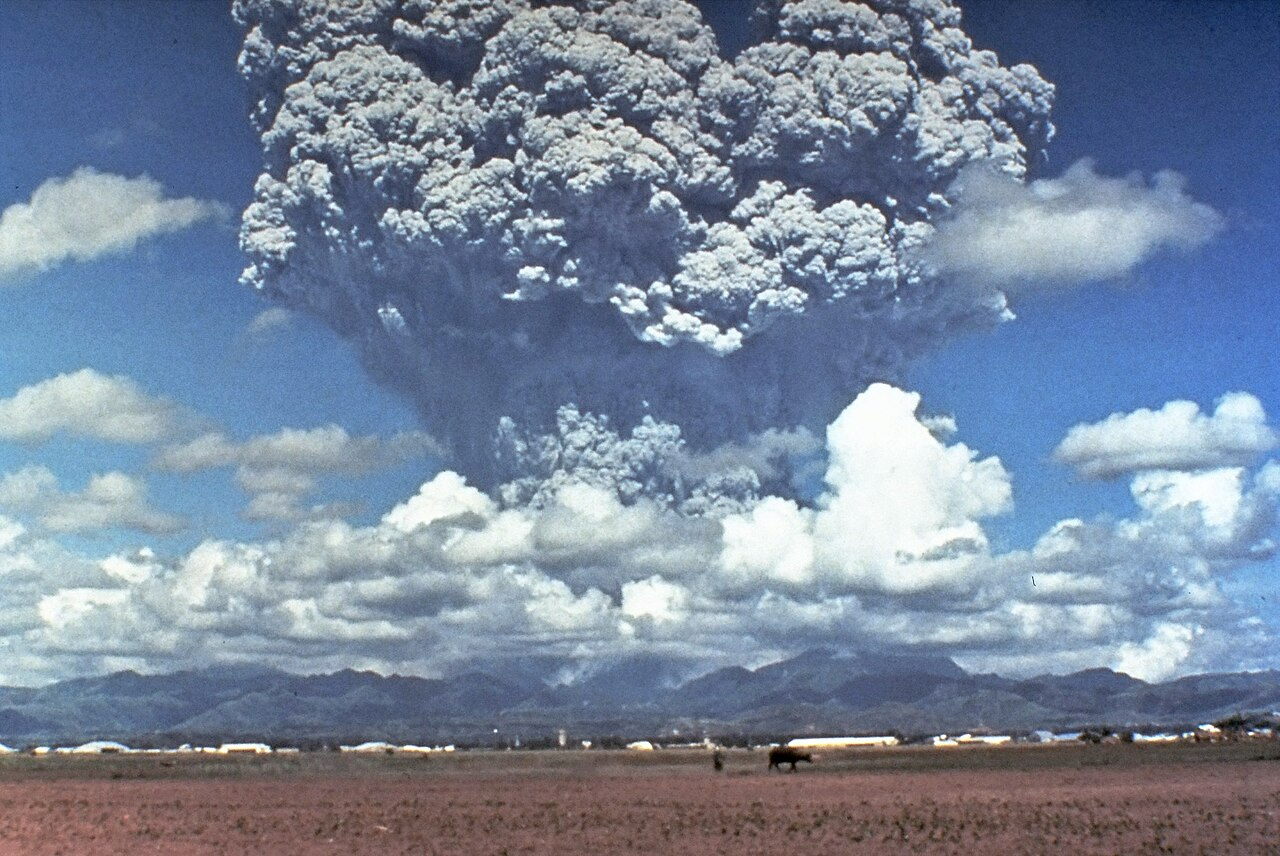
\includegraphics[height=4.5cm]{images/book1/g7-pinatubo.jpg}

{\small Explosiva: a coluna eruptiva do monte Pinatubo, Filipinas,
12~de~junho~de~1991. Foto: Dave Harlow, USGS.}
\end{minipage}\par\medskip


{\small As duas fotografias estão em domínio público (via Wikimedia
Commons).}
% ledger: commons:lava-fountain, commons:pinatubo
\label{fig:g7:volcanoes:two-photos}
\end{omfigure}

O que faz a diferença? Duas coisas: quão fluido é o \omterm{def:g7:volcanoes:magma}{magma}, e quanto gás
ele guarda.

\textbf{Fluido ou viscoso.} Alguns \omterm{def:g7:volcanoes:magma}{magmas} são fluidos, quase como mel
morno: é o caso do \omterm{def:g7:volcanoes:magma}{magma} que esfria e vira basalto escuro, como no Havaí.
Outros \omterm{def:g7:volcanoes:magma}{magmas} são grossos e viscosos, como mel frio ou pasta de dente.
Através de um \omterm{def:g7:volcanoes:magma}{magma} fluido, as bolhas de gás sobem com facilidade e
escapam na superfície, algumas de cada vez. Num \omterm{def:g7:volcanoes:magma}{magma} viscoso, as bolhas
ficam presas.

\textbf{Pouco ou muito gás.} Uma garrafa de água com gás guarda muito gás
dissolvido na água, mantido ali pela pressão dentro da garrafa fechada;
você não consegue vê-lo. Abra a garrafa, e a pressão cai: aparecem bolhas
por toda parte, e, se a garrafa foi sacudida, a espuma jorra para fora. O
\omterm{def:g7:volcanoes:magma}{magma}, bem fundo embaixo da terra, também guarda gás dissolvido sob alta
pressão. À medida que ele sobe, a pressão cai e o gás sai da solução em
forma de bolhas.
% ledger: usgs:volcanic-gases

Junte as duas coisas. Um \omterm{def:g7:volcanoes:magma}{magma} fluido com pouco gás deixa as suas bolhas
irem embora e sai como \omterm{def:g4:volcanoes-earthquakes-first-look:eruption}{lava} que corre: a \omterm{def:g4:volcanoes-earthquakes-first-look:eruption}{erupção} é efusiva. Um \omterm{def:g7:volcanoes:magma}{magma}
viscoso cheio de gás segura as suas bolhas até que elas incham tanto que
rasgam o \omterm{def:g7:volcanoes:magma}{magma} em farrapos: a \omterm{def:g4:volcanoes-earthquakes-first-look:eruption}{erupção} é explosiva. Os farrapos de \omterm{def:g7:volcanoes:magma}{magma}
espumoso se solidificam no ar e viram cinzas e pedra-pomes, uma \omterm{def:g3:stones-pebbles-sand:rock}{rocha} tão
cheia de bolhas que consegue flutuar.

\begin{example}[Pinatubo, 1991: o refrigerante sem gás e o refrigerante sacudido]\label{ex:g7:volcanoes:pinatubo}
% ledger: usgs:pinatubo-1991
Em junho~de~1991, o primeiro \omterm{def:g7:volcanoes:magma}{magma} chegou à superfície do monte Pinatubo,
nas Filipinas. No caminho para cima, ele tinha perdido a maior parte do seu
gás, ``como uma garrafa de refrigerante que perdeu o gás'', nas palavras
dos cientistas que observavam. Ele saiu devagar e se empilhou num monte
sobre a \omterm{def:g7:volcanoes:vent}{boca}: nenhuma explosão. Depois, em 12~de~junho, um \omterm{def:g7:volcanoes:magma}{magma} ainda
cheio de gás chegou à superfície e explodiu --- a coluna da fotografia
acima. Em 15~de~junho, chegou um \omterm{def:g7:volcanoes:magma}{magma} ainda mais rico em gás, e o \omterm{def:g4:volcanoes-earthquakes-first-look:volcano}{vulcão}
teve uma das maiores \omterm{def:g4:volcanoes-earthquakes-first-look:eruption}{erupções} do século XX: ele lançou mais de cinco
quilômetros cúbicos de \omterm{def:g3:stones-pebbles-sand:rock}{rocha} e de cinzas, a sua \omterm{def:g4:clouds-rain-snow:cloud}{nuvem} de cinzas subiu a
\qty{35}{km} de altura, e o alto da \omterm{def:g1:landscapes-around-us:landform}{montanha} desabou numa depressão de
\qty{2.5}{km} de largura. O mesmo \omterm{def:g4:volcanoes-earthquakes-first-look:volcano}{vulcão}, a mesma semana: o gás fez a
diferença.
\end{example}

A forma de um \omterm{def:g4:volcanoes-earthquakes-first-look:volcano}{vulcão} guarda a memória das suas \omterm{def:g4:volcanoes-earthquakes-first-look:eruption}{erupções}. A \omterm{def:g4:volcanoes-earthquakes-first-look:eruption}{lava} fluida
corre longe antes de endurecer, então, camada após camada, ela constrói
uma \omterm{def:g1:landscapes-around-us:landform}{montanha} larga de encostas suaves, com a forma do escudo de um
guerreiro deitado no chão: um \emph{vulcão-escudo}. O Mauna Loa, no Havaí,
é um deles. A \omterm{def:g4:volcanoes-earthquakes-first-look:eruption}{lava} viscosa e as cinzas se empilham perto da \omterm{def:g7:volcanoes:vent}{boca}, num cone
íngreme feito de camadas de \omterm{def:g4:volcanoes-earthquakes-first-look:eruption}{lava} e de cinzas: um \emph{estratovulcão}
(\emph{estrato} quer dizer camada). O monte Santa Helena e o Pinatubo são
dois deles.

\begin{omfigure}
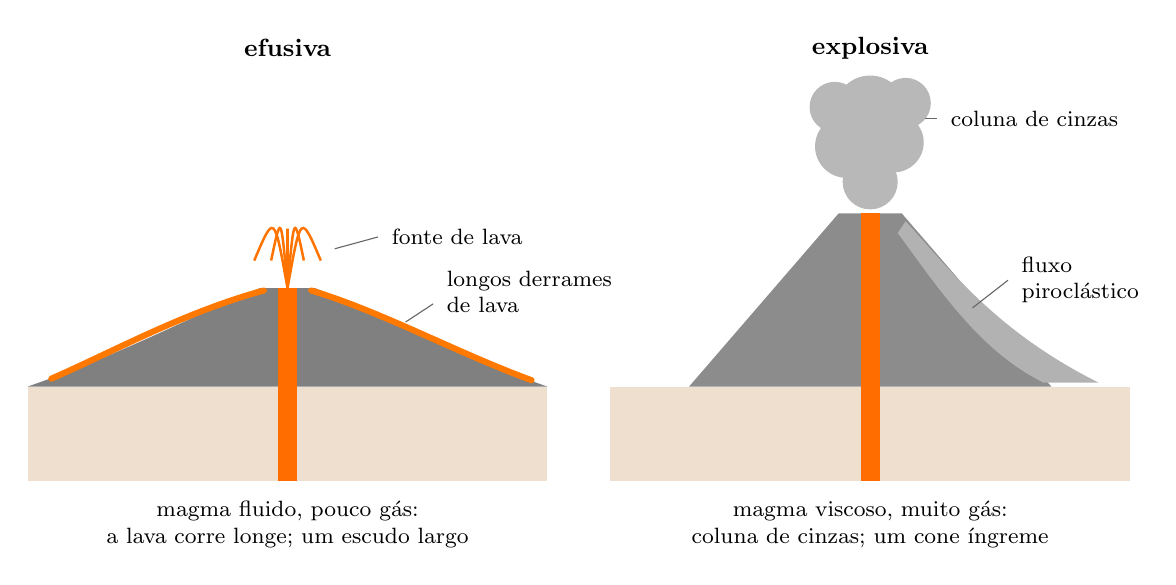
\begin{tikzpicture}[font=\small, x=1cm, y=1cm]
  % --- left: effusive, a shield
  \begin{scope}
    \fill[brown!25] (-3.3,-1.2) rectangle (3.3,0);
    \fill[black!50] (-3.3,0) .. controls (-2.0,0.45) and (-1.0,1.0) .. (-0.35,1.25)
      -- (0.35,1.25) .. controls (1.0,1.0) and (2.0,0.45) .. (3.3,0) -- cycle;
    \fill[orange!85!red] (-0.12,-1.2) rectangle (0.12,1.25);
    % fountain
    \foreach \a in {-25,-12,0,12,25}
      \draw[orange!90!red, line width=0.9pt] (0,1.25) .. controls ({0.4*sin(\a)},2.2) .. ({1.0*sin(\a)},1.6);
    % lava flows far down the gentle slopes
    \draw[orange!95!red, line width=2.2pt, line cap=round] (0.3,1.22) .. controls (1.2,0.95) and (2.1,0.45) .. (3.1,0.08);
    \draw[orange!95!red, line width=2.2pt, line cap=round] (-0.3,1.22) .. controls (-1.3,0.95) and (-2.2,0.45) .. (-3.0,0.1);
    \node[font=\small\bfseries] at (0,4.3) {efusiva};
    \node[align=center, font=\footnotesize] at (0,-1.75) {magma fluido, pouco gás:\\a lava corre longe; um escudo largo};
    \node[anchor=west, font=\footnotesize] at (1.2,1.9) {fonte de lava};
    \draw[black!60] (1.15,1.9) -- (0.6,1.75);
    \node[anchor=west, font=\footnotesize, align=left] at (1.9,1.2) {longos derrames\\de lava};
    \draw[black!60] (1.85,1.05) -- (1.5,0.82);
  \end{scope}
  % --- right: explosive, a steep cone
  \begin{scope}[xshift=7.4cm]
    \fill[brown!25] (-3.3,-1.2) rectangle (3.3,0);
    \fill[black!45] (-2.3,0) -- (-0.4,2.2) -- (0.4,2.2) -- (2.3,0) -- cycle;
    \fill[orange!85!red] (-0.12,-1.2) rectangle (0.12,2.2);
    \foreach \x/\y/\r in {0/2.6/0.35, -0.3/3.05/0.4, 0.3/3.1/0.38, 0/3.5/0.45, -0.45/3.55/0.32, 0.45/3.6/0.32}
      \fill[black!28] (\x,\y) circle (\r);
    % pyroclastic flow down the flank
    \fill[black!30] (0.45,2.1) .. controls (1.0,1.5) and (1.6,0.7) .. (2.9,0.05)
      -- (2.2,0.05) .. controls (1.4,0.45) and (0.9,1.2) .. (0.35,1.95) -- cycle;
    \node[font=\small\bfseries] at (0,4.3) {explosiva};
    \node[align=center, font=\footnotesize] at (0,-1.75) {magma viscoso, muito gás:\\coluna de cinzas; um cone íngreme};
    \node[anchor=west, font=\footnotesize] at (0.9,3.4) {coluna de cinzas};
    \draw[black!60] (0.85,3.4) -- (0.7,3.4);
    \node[anchor=west, font=\footnotesize, align=left] at (1.8,1.35) {fluxo\\piroclástico};
    \draw[black!60] (1.75,1.35) -- (1.3,1.0);
  \end{scope}
\end{tikzpicture}

{\small Os dois tipos de \omterm{def:g4:volcanoes-earthquakes-first-look:eruption}{erupção} e os \omterm{def:g4:volcanoes-earthquakes-first-look:volcano}{vulcões} que eles constroem (desenhos,
fora de escala).}
\label{fig:g7:volcanoes:two-kinds}
\end{omfigure}

\begin{method}[Efusiva ou explosiva? Quatro pistas]\label{met:g7:volcanoes:clues}
Para saber, a partir de uma descrição ou de uma fotografia, que tipo de
\omterm{def:g4:volcanoes-earthquakes-first-look:eruption}{erupção} um \omterm{def:g4:volcanoes-earthquakes-first-look:volcano}{vulcão} tem, procure estas pistas.
\begin{enumerate}
  \item \emph{O que sai?} \omterm{def:g4:volcanoes-earthquakes-first-look:eruption}{Lava} que corre ou jorra em fontes: efusiva. Uma
        coluna de cinzas, pedaços de \omterm{def:g3:stones-pebbles-sand:rock}{rocha} lançados: explosiva.
  \item \emph{A forma do \omterm{def:g4:volcanoes-earthquakes-first-look:volcano}{vulcão}.} Uma \omterm{def:g1:landscapes-around-us:landform}{montanha} larga de encostas suaves:
        \omterm{def:g4:volcanoes-earthquakes-first-look:eruption}{erupções} sobretudo efusivas. Um cone íngreme: muitas vezes
        explosivas.
  \item \emph{O \omterm{def:g7:volcanoes:magma}{magma}.} Fluido, pouco gás: efusiva. Viscoso, muito gás:
        explosiva.
  \item \emph{As \omterm{def:g3:stones-pebbles-sand:rock}{rochas} deixadas para trás.} Derrames de \omterm{def:g4:volcanoes-earthquakes-first-look:eruption}{lava} escuros e
        maciços: efusiva. Camadas de cinzas e de pedra-pomes: explosiva.
\end{enumerate}
\end{method}

\begin{example}[Usar as pistas]\label{ex:g7:volcanoes:clues}
Um viajante descreve um \omterm{def:g4:volcanoes-earthquakes-first-look:volcano}{vulcão}: ``uma \omterm{def:g1:landscapes-around-us:landform}{montanha} enorme, suavemente
arredondada, com derrames de \omterm{def:g4:volcanoes-earthquakes-first-look:eruption}{lava} negra por toda parte nas suas encostas,
alguns deles com só alguns anos''. A pista~2 (encostas suaves) e a
pista~4 (derrames de \omterm{def:g4:volcanoes-earthquakes-first-look:eruption}{lava} escuros) apontam as duas para \omterm{def:g7:volcanoes:eruption-types}{erupções efusivas}:
é um vulcão-escudo, como o Mauna Loa.
\end{example}

\begin{inthelab}[Um vulcão numa garrafa (em aula, com a professora)]
A professora pega duas garrafas fechadas de água com gás. Uma ficou parada;
a outra foi sacudida de leve. As duas são abertas ao ar livre, em cima de
uma bacia, apontadas para longe de todo mundo. A garrafa parada chia e
deixa subir algumas bolhas; a sacudida explode em espuma que jorra para
fora. Que garrafa é como o \omterm{def:g7:volcanoes:magma}{magma} do Havaí, e qual é como o do Pinatubo?
Depois, jogue um pedaço de pedra-pomes e um \omterm{def:g3:stones-pebbles-sand:pebble}{seixo} numa tigela de água: a
pedra-pomes flutua. Observe-a com uma lupa: ela é cheia de buracos, as
bolhas de gás congeladas na \omterm{def:g3:stones-pebbles-sand:rock}{rocha} quando o \omterm{def:g7:volcanoes:magma}{magma} explodiu.
\end{inthelab}

\section{O que sai de um vulcão}

Uma \omterm{def:g4:volcanoes-earthquakes-first-look:eruption}{erupção} lança muito mais que \omterm{def:g4:volcanoes-earthquakes-first-look:eruption}{lava}: gases, cinzas, pedaços de \omterm{def:g3:stones-pebbles-sand:rock}{rocha} e,
nos piores casos, avalanches de cinzas quentes.

O gás mais abundante, de longe, é o vapor de água. As grandes \omterm{def:g4:volcanoes-earthquakes-first-look:eruption}{erupções}
liberam quantidades enormes de gás em pouco tempo: num único dia de 1991,
o Pinatubo deve ter mandado mais de 250~milhões de toneladas de gás para a
alta atmosfera.
% ledger: usgs:volcanic-gases

\begin{definition}[Fluxo piroclástico]\label{def:g7:volcanoes:pyroclastic-flow}
Um \emph{fluxo piroclástico}\index{fluxo piroclastico@fluxo piroclástico} é uma avalanche rápida de
gás quente, de cinzas e de pedaços de \omterm{def:g3:stones-pebbles-sand:rock}{rocha}, de grãos de poeira a
matacões, que desce as encostas de um \omterm{def:g4:volcanoes-earthquakes-first-look:volcano}{vulcão} a toda a velocidade durante
uma \omterm{def:g7:volcanoes:eruption-types}{erupção explosiva}. (\emph{Piro} quer dizer fogo, e \emph{clástico}
quer dizer feito de pedaços quebrados.)
\end{definition}

Os \omterm{def:g7:volcanoes:pyroclastic-flow}{fluxos piroclásticos} em geral andam a mais de \qty{80}{km/h}, e as
\omterm{def:g3:stones-pebbles-sand:rock}{rochas} e os gases dentro deles em geral estão entre 200 e
\qty{700}{\degreeCelsius}. Em geral, eles seguem os \omterm{def:g1:landscapes-around-us:landform}{vales}, como a água, e derrubam, queimam ou
soterram quase tudo no seu caminho. Em 18~de~maio~de~1980, os \omterm{def:g7:volcanoes:pyroclastic-flow}{fluxos
piroclásticos} do monte Santa Helena correram a 80 a \qty{130}{km/h}, a uma
temperatura de pelo menos \qty{700}{\degreeCelsius}, e chegaram a
\qty{8}{km} da \omterm{def:g7:volcanoes:vent}{cratera}.
% ledger: usgs:pyroclastic-flows, usgs:msh-flows, usgs:msh-reach

A tabela resume os produtos de um \omterm{def:g4:volcanoes-earthquakes-first-look:volcano}{vulcão}.

\begin{center}
\small
\begin{tabular}{|p{0.2\linewidth}|p{0.4\linewidth}|p{0.3\linewidth}|}
\hline
\textbf{produto} & \textbf{o que é} & \textbf{o perigo} \\
\hline
derrame de \omterm{def:g4:volcanoes-earthquakes-first-look:eruption}{lava} & \omterm{def:g3:stones-pebbles-sand:rock}{rocha} derretida que corre pelo chão e depois endurece & queima e soterra o que encontra, mas em geral é lento o bastante para as pessoas saírem do caminho \\
\hline
cinzas & pedacinhos de \omterm{def:g3:stones-pebbles-sand:rock}{rocha} e de vidro, lançados no ar & caem longe; os telhados desabam com o seu peso; danificam os aviões \\
\hline
bombas vulcânicas & pedaços de \omterm{def:g4:volcanoes-earthquakes-first-look:eruption}{lava} lançados, que endurecem enquanto voam & esmagam o que atingem, perto da \omterm{def:g7:volcanoes:vent}{boca} \\
\hline
gases & sobretudo vapor de água, depois gás carbônico e dióxido de enxofre & alguns são venenosos; o gás carbônico se acumula nas depressões \\
\hline
\omterm{def:g7:volcanoes:pyroclastic-flow}{fluxo piroclástico} & uma avalanche de cinzas, de \omterm{def:g3:stones-pebbles-sand:rock}{rocha} e de gás quentes & o mais mortal: rápido e quente demais para se escapar dele \\
\hline
fluxo de lama & cinzas e \omterm{def:g3:stones-pebbles-sand:rock}{rocha} misturadas com a água da \omterm{def:g4:clouds-rain-snow:precipitation}{chuva} ou da \omterm{def:g4:clouds-rain-snow:precipitation}{neve} derretida & desce os \omterm{def:g1:landscapes-around-us:landform}{vales} a toda a velocidade, às vezes longe do \omterm{def:g4:volcanoes-earthquakes-first-look:volcano}{vulcão} \\
\hline
\end{tabular}
\end{center}
% ledger: usgs:lava-flows, usgs:volcanic-gases, usgs:pyroclastic-flows, usgs:pinatubo-1991, usgs:msh-flows

\begin{method}[Quanto tempo leva?]\label{met:g7:volcanoes:time}
Para descobrir quanto tempo algo que se move a uma velocidade conhecida
leva para percorrer uma distância, divida a distância pela velocidade:
\[
\text{tempo} = \frac{\text{distância}}{\text{velocidade}}.
\]
Com uma distância em quilômetros e uma velocidade em quilômetros por hora,
o tempo sai em horas; multiplique por 60 para obter minutos.
\end{method}

\begin{example}[Uma corrida contra um fluxo piroclástico]\label{ex:g7:volcanoes:race}
Um \omterm{def:g7:volcanoes:pyroclastic-flow}{fluxo piroclástico} que anda a \qty{120}{km/h} vai na direção de uma
aldeia a \qty{6}{km} \omterm{def:g1:landscapes-around-us:landform}{vale} abaixo. Ele leva $6 \div 120 = 0.05$~hora, ou
seja, $0.05 \times 60 = 3$~minutos. Três minutos: ninguém consegue sair do
\omterm{def:g1:landscapes-around-us:landform}{vale} correndo, nem mesmo de carro, a tempo. As pessoas só estão seguras se
tiverem partido \emph{antes} da \omterm{def:g4:volcanoes-earthquakes-first-look:eruption}{erupção}.
\end{example}

\begin{remark}[Os fluxos de lama: o perigo que vem depois]\label{rem:g7:volcanoes:mudflows}
% ledger: usgs:msh-flows, usgs:pinatubo-lahars
Uma \omterm{def:g4:volcanoes-earthquakes-first-look:eruption}{erupção} deixa as encostas cobertas de cinzas soltas. Quando a \omterm{def:g4:clouds-rain-snow:precipitation}{chuva} cai
sobre elas, ou quando o calor derrete a \omterm{def:g4:clouds-rain-snow:precipitation}{neve} e o gelo do cume, as cinzas
viram fluxos de lama que descem os \omterm{def:g1:landscapes-around-us:landform}{vales} a toda a velocidade. Em
18~de~maio~de~1980, os fluxos de lama do monte Santa Helena danificaram
27~pontes e quase 200~casas. Em volta do Pinatubo, as \omterm{def:g4:clouds-rain-snow:precipitation}{chuvas} fortes dos
anos seguintes transformaram as cinzas em fluxos de lama gigantes que
soterraram aldeias inteiras: eles causaram mais estragos que a própria
\omterm{def:g4:volcanoes-earthquakes-first-look:eruption}{erupção}.
\end{remark}


\section{Onde ficam os vulcões?}

A Smithsonian Institution, em Washington, mantém uma lista de todos os
\omterm{def:g4:volcanoes-earthquakes-first-look:volcano}{vulcões} que sabemos que entraram em \omterm{def:g4:volcanoes-earthquakes-first-look:eruption}{erupção} nos últimos 12\,000 anos:
1\,214 \omterm{def:g4:volcanoes-earthquakes-first-look:volcano}{vulcões}, em terra e embaixo do \omterm{def:g2:water-on-earth:ocean}{mar}. Para cada um, a lista diz onde
ele fica em relação às \omterm{def:g7:plate-tectonics:plate}{placas}. O \omterm{def:g2:drawing-to-map:map}{mapa} abaixo os colore desse jeito.
% ledger: data:gvp (counts computed in figdata/grade-7/volcano_settings.py)

\begin{omfigure}
\begin{tikzpicture}
\begin{axis}[ommap, width=\linewidth, xtick={-180,-90,...,180}, ytick={-60,0,60},
  legend style={at={(0.02,0.04)}, anchor=south west, font=\scriptsize,
  fill=white, fill opacity=0.85, text opacity=1, draw=black!40}, legend cell align=left]
\addplot[fill=omLithAlluv, draw=black!45, line width=0.2pt, forget plot] table {figdata/out/shared-geo-land.dat};
\addplot[omRidge!60, line width=0.5pt, forget plot] table {figdata/out/shared-geo-school-ridge.dat};
\addplot[omTrench!60, line width=0.5pt, forget plot] table {figdata/out/shared-geo-school-subduction.dat};
\addplot[only marks, mark=triangle*, mark size=1.3pt, omTrench, forget plot] table {figdata/out/grade-7-volcano_settings-map-sub.dat};
\addplot[only marks, mark=triangle*, mark size=1.3pt, omRidge, forget plot] table {figdata/out/grade-7-volcano_settings-map-rift.dat};
\addplot[only marks, mark=*, mark size=1.4pt, orange!90!black, forget plot] table {figdata/out/grade-7-volcano_settings-map-intra.dat};
\addlegendimage{only marks, mark=triangle*, mark size=1.6pt, omTrench}
\addlegendentry{onde uma placa afunda embaixo de outra}
\addlegendimage{only marks, mark=triangle*, mark size=1.6pt, omRidge}
\addlegendentry{onde as placas se afastam}
\addlegendimage{only marks, mark=*, mark size=1.6pt, orange!90!black}
\addlegendentry{dentro de uma placa}
\end{axis}
\end{tikzpicture}

{\small Os \omterm{def:g4:volcanoes-earthquakes-first-look:volcano}{vulcões} ativos nos últimos 12\,000 anos, coloridos conforme o
lugar onde ficam. Linhas claras: os \omterm{def:g7:plate-tectonics:plate-boundary}{limites de placas} onde as \omterm{def:g7:plate-tectonics:plate}{placas} se
afastam (em vermelho) e onde uma \omterm{def:g7:plate-tectonics:plate}{placa} afunda embaixo de outra (em azul).
Dados: Smithsonian Global Volcanism Program; limites segundo P.~Bird
(2003); litorais de Natural Earth.}
% ledger: data:gvp, data:pb2002, data:ne-land
\label{fig:g7:volcanoes:map}
\end{omfigure}

\begin{omfigure}
\begin{tikzpicture}
  \begin{axis}[xbar, width=0.72\linewidth, height=3.6cm, bar width=8pt,
      xmin=0, xmax=1000, ymin=-0.6, ymax=3.6, y dir=reverse,
      ytick={0,...,3}, yticklabels={onde uma placa afunda embaixo de outra,onde as placas se afastam,dentro de uma placa,desconhecido},
      xlabel={número de vulcões},
      axis x line=bottom, axis y line=left, axis line style={-},
      tick label style={font=\scriptsize}, label style={font=\small},
      nodes near coords, nodes near coords style={font=\scriptsize, anchor=west},
      point meta=explicit symbolic, enlarge y limits=false, clip=false]
    \addplot[fill=black!30, draw=black!60] table[x=n, y=idx, meta=n] {figdata/out/grade-7-volcano_settings.dat};
  \end{axis}
\end{tikzpicture}

{\small Quantos dos 1\,214 \omterm{def:g4:volcanoes-earthquakes-first-look:volcano}{vulcões} ficam em cada situação.}
% ledger: data:gvp (figdata/grade-7/volcano_settings.py, main table)
\label{fig:g7:volcanoes:counts}
\end{omfigure}

\begin{proposition}[A maioria dos vulcões fica nos limites de placas]\label{prop:g7:volcanoes:where}
% ledger: data:gvp (counts computed in figdata/grade-7/volcano_settings.py)
Dos 1\,214 \omterm{def:g4:volcanoes-earthquakes-first-look:volcano}{vulcões} ativos nos últimos 12\,000 anos, 838 (69~\%) ficam onde
uma \omterm{def:g7:plate-tectonics:plate}{placa} afunda embaixo de outra e 221 (18~\%) onde as \omterm{def:g7:plate-tectonics:plate}{placas} se afastam;
149 (12~\%) ficam dentro de uma \omterm{def:g7:plate-tectonics:plate}{placa}, longe das suas bordas. Para os 6
últimos (0.5~\%), a situação é desconhecida.
\end{proposition}

\textbf{Onde as \omterm{def:g7:plate-tectonics:plate}{placas} se afastam.} Ao longo das dorsais oceânicas, e em
riftes como o que está rasgando a África Oriental, as \omterm{def:g7:plate-tectonics:plate}{placas} se afastam
uma da outra. O \omterm{def:g7:volcanoes:magma}{magma} sobe do \omterm{def:g6:inside-the-earth:layers}{manto} para as fendas que se alargam e as
preenche: forma-se \omterm{def:g6:inside-the-earth:layers}{crosta} nova. A maioria das dorsais fica embaixo do \omterm{def:g2:water-on-earth:ocean}{mar}, mas a Islândia fica
bem em cima da dorsal mesoatlântica: ali, esses \omterm{def:g4:volcanoes-earthquakes-first-look:volcano}{vulcões} podem ser vistos
em terra. O seu \omterm{def:g7:volcanoes:magma}{magma} é sobretudo basalto fluido, e as suas \omterm{def:g4:volcanoes-earthquakes-first-look:eruption}{erupções} são
sobretudo efusivas.
% ledger: usgs:arc-magma, usgs:iceland, usgs:east-africa

\textbf{Onde uma \omterm{def:g7:plate-tectonics:plate}{placa} afunda embaixo de outra.} Mais de dois \omterm{def:g4:volcanoes-earthquakes-first-look:volcano}{vulcões} em
cada três ficam aqui, ao longo de linhas que seguem as bordas do \omterm{def:g2:water-on-earth:ocean}{oceano}
Pacífico --- o ``Círculo de Fogo'' --- e em alguns outros lugares. Lá no
fundo, ao longo da \omterm{def:g7:plate-tectonics:plate}{placa} que afunda, uma parte da \omterm{def:g3:stones-pebbles-sand:rock}{rocha} derrete em parte;
os cientistas ainda discutem exatamente qual \omterm{def:g3:stones-pebbles-sand:rock}{rocha} derrete, a \omterm{def:g7:plate-tectonics:plate}{placa} que
afunda ou a \omterm{def:g7:plate-tectonics:plate}{placa} de cima, ou as duas. O \omterm{def:g7:volcanoes:magma}{magma} que sobe ali muitas vezes é
viscoso e cheio de gás: são os \omterm{def:g4:volcanoes-earthquakes-first-look:volcano}{vulcões} explosivos, como o monte Santa
Helena e o Pinatubo. Os dados mostram isso: dos 660 cones íngremes
(estratovulcões) da lista, 564 --- ou seja, 85~\% --- ficam onde uma \omterm{def:g7:plate-tectonics:plate}{placa}
afunda embaixo de outra.
% ledger: usgs:arc-magma, data:gvp (figdata/grade-7/volcano_settings.py, part strato)

\textbf{Dentro de uma \omterm{def:g7:plate-tectonics:plate}{placa}.} Alguns \omterm{def:g4:volcanoes-earthquakes-first-look:volcano}{vulcões} ficam longe de qualquer
limite. Os mais famosos são os do Havaí, no meio do \omterm{def:g2:water-on-earth:ocean}{oceano} Pacífico, a mais
de \qty{3200}{km} da borda mais próxima de uma \omterm{def:g7:plate-tectonics:plate}{placa}.
% ledger: usgs:hawaii-hotspot

\begin{definition}[Ponto quente]\label{def:g7:volcanoes:hotspot}
Um \emph{ponto quente}\index{ponto quente} é um lugar, bem fundo no \omterm{def:g6:inside-the-earth:layers}{manto}, que
continua quente durante milhões de anos e alimenta sem parar de \omterm{def:g7:volcanoes:magma}{magma} os
\omterm{def:g4:volcanoes-earthquakes-first-look:volcano}{vulcões} da superfície, mesmo longe das bordas das \omterm{def:g7:plate-tectonics:plate}{placas}.
\end{definition}

O \omterm{def:g7:volcanoes:hotspot}{ponto quente} fica onde está, enquanto a \omterm{def:g7:plate-tectonics:plate}{placa} acima dele se move. Um
\omterm{def:g4:volcanoes-earthquakes-first-look:volcano}{vulcão} cresce acima do \omterm{def:g7:volcanoes:hotspot}{ponto quente}; depois, a \omterm{def:g7:plate-tectonics:plate}{placa} em movimento o leva
embora, e ele morre, enquanto um novo \omterm{def:g4:volcanoes-earthquakes-first-look:volcano}{vulcão} cresce sobre o \omterm{def:g7:volcanoes:hotspot}{ponto quente},
atrás dele. Com o tempo, a \omterm{def:g7:plate-tectonics:plate}{placa} leva toda uma fileira de \omterm{def:g4:volcanoes-earthquakes-first-look:volcano}{vulcões}, o mais
velho mais longe do \omterm{def:g7:volcanoes:hotspot}{ponto quente}. É exatamente o que vemos no Havaí: as
\omterm{def:g3:stones-pebbles-sand:rock}{rochas} mais velhas da ilha de Kauai, na ponta noroeste das ilhas
habitadas, têm cerca de 5.5~milhões de anos e estão muito desgastadas pela
\omterm{def:g4:clouds-rain-snow:precipitation}{chuva} e pelas ondas; na Ilha Grande, na ponta sudeste, as \omterm{def:g3:stones-pebbles-sand:rock}{rochas} mais
velhas da superfície têm menos de 0.7~milhão de anos, e ainda sai \omterm{def:g4:volcanoes-earthquakes-first-look:eruption}{lava}
nova.
% ledger: usgs:hawaii-hotspot

\begin{history}[Um geofísico e uma fileira de ilhas]
% ledger: usgs:hawaii-hotspot
Por que uma cadeia de ilhas vulcânicas surgiria no meio da maior \omterm{def:g7:plate-tectonics:plate}{placa} da
Terra? Em 1963, o geofísico canadense J.~Tuzo Wilson propôs uma resposta.
As ilhas do Havaí, sugeriu ele, formam uma fileira porque a \omterm{def:g7:plate-tectonics:plate}{placa} do
Pacífico se move sobre uma fonte de calor profunda e fixa no \omterm{def:g6:inside-the-earth:layers}{manto}, que
derrete em parte a \omterm{def:g7:plate-tectonics:plate}{placa} acima dela. Se ele tivesse razão, as ilhas
deveriam ser mais velhas e mais desgastadas quanto mais longe ficassem dos
\omterm{def:g4:volcanoes-earthquakes-first-look:volcano}{vulcões} ativos da Ilha Grande. As idades das suas \omterm{def:g3:stones-pebbles-sand:rock}{rochas} mostram exatamente isso. Uma única ideia explicou ao mesmo tempo a fileira e a ordem das idades.
(Wilson também é o cientista que descobriu os \omterm{def:g7:plate-tectonics:plate-boundary}{limites transformantes}, onde
as \omterm{def:g7:plate-tectonics:plate}{placas} deslizam uma ao lado da outra.)
\end{history}

\begin{omfigure}
\begin{tikzpicture}[font=\small, x=1cm, y=1cm]
  % sea, plate and mantle
  \fill[omSea!45] (-6.2,0) rectangle (6.2,1.0);
  \fill[orange!12] (-6.2,-3.4) rectangle (6.2,-1.0);
  \fill[brown!35] (-6.2,-1.0) rectangle (6.2,0);
  \draw[omSea!80!black, line width=0.5pt] (-6.2,1.0) -- (6.2,1.0);
  \node[font=\footnotesize] at (-4.6,-0.5) {placa do Pacífico};
  % the hotspot plume, fixed in the mantle, and the magma rising to the volcano
  \fill[orange!80!red] (4.0,-3.4) .. controls (3.6,-2.4) .. (3.75,-1.0) -- (4.25,-1.0) .. controls (4.4,-2.4) .. (4.0,-3.4) -- cycle;
  \node[anchor=west, align=left, font=\footnotesize] at (4.5,-2.5) {ponto quente:\\fica no lugar};
  % volcanoes rise from the sea floor; youngest over the hotspot
  \fill[black!55] (2.3,0) .. controls (3.2,1.2) .. (3.75,1.85) -- (4.25,1.85) .. controls (4.8,1.2) .. (5.7,0) -- cycle;
  \fill[orange!80!red] (3.93,-1.0) rectangle (4.07,1.85);
  \fill[black!45] (-0.4,0) .. controls (0.4,0.9) .. (0.9,1.3) -- (1.3,1.3) .. controls (1.8,0.9) .. (2.6,0) -- cycle;
  \fill[black!35] (-3.2,0) .. controls (-2.5,0.6) .. (-2.1,0.8) -- (-1.7,0.8) .. controls (-1.3,0.6) .. (-0.6,0) -- cycle;
  \fill[black!28] (-5.8,0) .. controls (-5.2,0.4) .. (-4.9,0.5) -- (-4.6,0.5) .. controls (-4.3,0.4) .. (-3.6,0) -- cycle;
  % labels
    \node[align=center, font=\footnotesize, anchor=south] at (4.3,1.95) {vulcão ativo\\(Ilha Grande: menos\\de 0.7 milhão de anos)};
  \node[align=center, font=\footnotesize, anchor=south] at (0.7,1.4) {ilha velha e desgastada\\(Kauai: cerca de\\5.5 milhões de anos)};
  \node[align=center, font=\footnotesize] at (-1.9,1.5) {vulcão mais velho,\\embaixo das ondas};
  \node[align=center, font=\footnotesize] at (-4.75,1.3) {mais velho ainda,\\afundando};
  \node[font=\footnotesize] at (5.75,0.55) {mar};
  \node[font=\footnotesize] at (-4.3,-2.2) {manto};
  % plate motion
  \draw[-{Stealth[length=3mm]}, line width=1.2pt] (2.2,-0.62) -- (-1.8,-0.62);
  \node[font=\footnotesize] at (0.2,-0.28) {a placa se move para o noroeste};
    \node[font=\footnotesize\bfseries] at (-5.8,-3.1) {NO};
  \node[font=\footnotesize\bfseries] at (5.8,-3.1) {SE};
\end{tikzpicture}

{\small Uma \omterm{def:g7:plate-tectonics:plate}{placa} que se move sobre um \omterm{def:g7:volcanoes:hotspot}{ponto quente} (um desenho, fora de
escala; as ilhas do meio foram deixadas de fora). O \omterm{def:g4:volcanoes-earthquakes-first-look:volcano}{vulcão} sobre o \omterm{def:g7:volcanoes:hotspot}{ponto
quente} é jovem e ativo; a \omterm{def:g7:plate-tectonics:plate}{placa} leva os mais velhos para o noroeste, onde
eles morrem, se desgastam e por fim afundam embaixo das ondas.}
% ledger: usgs:hawaii-hotspot
\label{fig:g7:volcanoes:hotspot}
\end{omfigure}

\begin{omfigure}
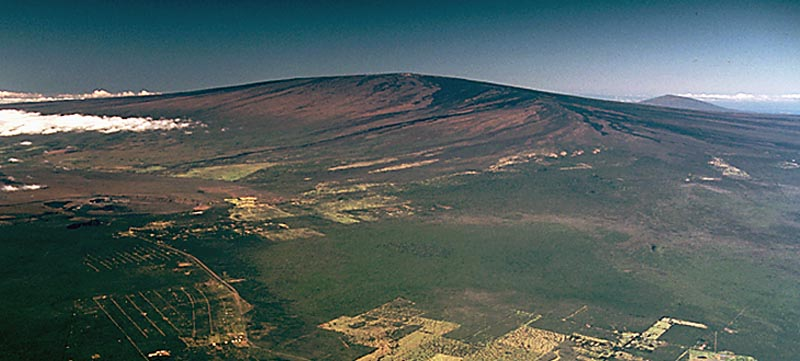
\includegraphics[width=0.8\linewidth]{images/book1/g7-mauna-loa.jpg}

{\small O Mauna Loa, um vulcão-escudo na Ilha Grande do Havaí, visto do ar:
uma \omterm{def:g1:landscapes-around-us:landform}{montanha} enorme de encostas suaves, construída por milhares de
derrames de \omterm{def:g4:volcanoes-earthquakes-first-look:eruption}{lava} fluida. Foto: J.~D. Griggs, U.S. Geological Survey, 1985
(domínio público, via Wikimedia Commons).}
% ledger: commons:mauna-loa
\label{fig:g7:volcanoes:mauna-loa}
\end{omfigure}

\section{Viver com os vulcões}

Muitas pessoas moram perto de \omterm{def:g4:volcanoes-earthquakes-first-look:volcano}{vulcões}: cerca de 3~milhões moravam na
região em volta do Pinatubo em 1991. Felizmente, uma grande \omterm{def:g4:volcanoes-earthquakes-first-look:eruption}{erupção} muitas
vezes dá sinais de aviso. O \omterm{def:g7:volcanoes:magma}{magma} que sobe empurra as \omterm{def:g3:stones-pebbles-sand:rock}{rochas} para os
lados: o chão racha e treme com pequenos \omterm{def:g4:volcanoes-earthquakes-first-look:earthquake}{terremotos}, as encostas incham,
gases escapam. No monte Santa Helena, os primeiros pequenos \omterm{def:g4:volcanoes-earthquakes-first-look:earthquake}{terremotos}
vieram em 16~de~março~de~1980; até 17~de~maio, tinha havido mais de
10\,000, e a face norte tinha inchado para fora pelo menos \qty{137}{m}.
Os cientistas mediram tudo isso e a área foi fechada; mesmo assim,
57~pessoas morreram em 18~de~maio.
% ledger: usgs:msh-lead-up, usgs:msh-flows

No Pinatubo, em 1991, os cientistas que observavam os \omterm{def:g4:volcanoes-earthquakes-first-look:earthquake}{terremotos}, os gases
e o inchaço do \omterm{def:g4:volcanoes-earthquakes-first-look:volcano}{vulcão} deram o alerta a tempo: as pessoas que moravam perto
do \omterm{def:g4:volcanoes-earthquakes-first-look:volcano}{vulcão} partiram, e pelo menos 5\,000 vidas foram salvas.
% ledger: usgs:pinatubo-1991 (central Luzon home to about 3 million people)

\begin{remark}[Nunca chegue perto de um vulcão em erupção]\label{rem:g7:volcanoes:safety}
Observar uma \omterm{def:g4:volcanoes-earthquakes-first-look:eruption}{erupção} é só para os lugares que as autoridades abriram ao
público. Os gases, as \omterm{def:g3:stones-pebbles-sand:rock}{rochas} que caem, a \omterm{def:g6:inside-the-earth:layers}{crosta} de \omterm{def:g4:volcanoes-earthquakes-first-look:eruption}{lava} fresca que se
quebra embaixo dos pés e os \omterm{def:g7:volcanoes:pyroclastic-flow}{fluxos piroclásticos} podem matar, muitas vezes
sem aviso. Os observatórios vulcanológicos publicam o que é seguro
visitar: siga-os sempre.
\end{remark}

\section{Exercícios}

\begin{exercise}[$\star$]\label{exo:g7:volcanoes:1}
Ligue cada palavra ao seu significado: \omterm{def:g7:volcanoes:magma}{magma}; \omterm{def:g4:volcanoes-earthquakes-first-look:eruption}{lava}; \omterm{def:g7:volcanoes:magma-chamber}{câmara magmática};
\omterm{def:g7:volcanoes:vent}{boca}; \omterm{def:g7:volcanoes:vent}{cratera}. (a) Uma depressão em forma de tigela no alto de um \omterm{def:g4:volcanoes-earthquakes-first-look:volcano}{vulcão}.
(b) \omterm{def:g3:stones-pebbles-sand:rock}{Rocha} derretida embaixo da terra. (c) Uma abertura por onde o \omterm{def:g7:volcanoes:magma}{magma}
sai. (d) \omterm{def:g3:stones-pebbles-sand:rock}{Rocha} derretida que saiu na superfície. (e) Um grande bolsão de
\omterm{def:g7:volcanoes:magma}{magma} a alguns quilômetros embaixo de um \omterm{def:g4:volcanoes-earthquakes-first-look:volcano}{vulcão}.
\end{exercise}

\begin{exercise}[$\star$]\label{exo:g7:volcanoes:2}
Efusiva ou explosiva? (a) \omterm{def:g1:landscapes-around-us:water}{Rios} de \omterm{def:g4:volcanoes-earthquakes-first-look:eruption}{lava} incandescente descem uma encosta
suave. (b) Uma coluna de cinzas sobe \qty{35}{km} no céu. (c) Uma fonte de
gotas incandescentes jorra de uma fenda. (d) Uma avalanche de cinzas e de
gás quentes desce um \omterm{def:g1:landscapes-around-us:landform}{vale} a toda a velocidade.
\end{exercise}

\begin{exercise}[$\star$]\label{exo:g7:volcanoes:3}
Verdadeiro ou falso? Corrija as falsas. (a) \omterm{def:g7:volcanoes:magma}{Magma} e \omterm{def:g4:volcanoes-earthquakes-first-look:eruption}{lava} são dois nomes da
mesma \omterm{def:g3:stones-pebbles-sand:rock}{rocha} derretida, embaixo da terra e na superfície. (b) O gás
vulcânico mais abundante é o gás carbônico. (c) Um \omterm{def:g7:volcanoes:pyroclastic-flow}{fluxo piroclástico} é um
\omterm{def:g1:landscapes-around-us:water}{rio} de \omterm{def:g4:volcanoes-earthquakes-first-look:eruption}{lava} líquida. (d) Os \omterm{def:g4:volcanoes-earthquakes-first-look:volcano}{vulcões} do Havaí ficam num \omterm{def:g7:plate-tectonics:plate-boundary}{limite de placas}.
\end{exercise}

\begin{exercise}[$\star$]\label{exo:g7:volcanoes:4}
Use a tabela das cores do brilho. (a) A \omterm{def:g4:volcanoes-earthquakes-first-look:eruption}{lava} brilha em amarelo: dê a sua
temperatura. (b) Um derrame que está endurecendo brilha em vermelho-escuro:
dê a sua temperatura. (c) Uma fotografia mostra \omterm{def:g4:volcanoes-earthquakes-first-look:eruption}{lava} laranja na frente de
um derrame e \omterm{def:g4:volcanoes-earthquakes-first-look:eruption}{lava} amarela perto da \omterm{def:g7:volcanoes:vent}{boca}. Onde é mais quente? Por quê?
\end{exercise}

\begin{exercise}[$\star\star$]\label{exo:g7:volcanoes:5}
Use o gráfico de barras dos 1\,214 \omterm{def:g4:volcanoes-earthquakes-first-look:volcano}{vulcões}. (a) Quantos \omterm{def:g4:volcanoes-earthquakes-first-look:volcano}{vulcões} ficam num
\omterm{def:g7:plate-tectonics:plate-boundary}{limite de placas} (onde as \omterm{def:g7:plate-tectonics:plate}{placas} se afastam, ou onde uma afunda embaixo de
outra)? (b) Que porcentagem de todos os \omterm{def:g4:volcanoes-earthquakes-first-look:volcano}{vulcões} isso representa?
(c) Verifique que as quatro porcentagens da proposição somam cerca de
100~\%.
\end{exercise}

\begin{exercise}[$\star\star$]\label{exo:g7:volcanoes:6}
Dos 660 cones íngremes (estratovulcões) da lista, 564 ficam onde uma \omterm{def:g7:plate-tectonics:plate}{placa}
afunda embaixo de outra, 62 onde as \omterm{def:g7:plate-tectonics:plate}{placas} se afastam e 33 dentro de uma
\omterm{def:g7:plate-tectonics:plate}{placa}. (a) Encontre a porcentagem de cones íngremes que ficam onde uma
\omterm{def:g7:plate-tectonics:plate}{placa} afunda embaixo de outra. (b) Quantos cones íngremes sobram para a
situação ``desconhecida''? (c) Use as quatro pistas: que tipo de \omterm{def:g4:volcanoes-earthquakes-first-look:eruption}{erupções}
devemos esperar ao longo do Círculo de Fogo?
\end{exercise}

\begin{exercise}[$\star\star$]\label{exo:g7:volcanoes:7}
No Kilauea, a \omterm{def:g4:volcanoes-earthquakes-first-look:eruption}{lava} sai da \omterm{def:g7:volcanoes:vent}{boca} a cerca de \qty{1170}{\degreeCelsius}. Num
túnel de \omterm{def:g4:volcanoes-earthquakes-first-look:eruption}{lava}, ela chegou ao \omterm{def:g2:water-on-earth:ocean}{mar}, a \qty{10}{km}, a cerca de
\qty{1140}{\degreeCelsius}. (a) Quantos graus ela esfriou? (b) Quantos
graus isso dá por quilômetro? (c) A \omterm{def:g4:volcanoes-earthquakes-first-look:eruption}{lava} ao ar livre esfria centenas de
graus por segundo na sua superfície. Explique por que a \omterm{def:g4:volcanoes-earthquakes-first-look:eruption}{lava} do túnel
continuou tão quente.
\end{exercise}

\begin{exercise}[$\star\star$]\label{exo:g7:volcanoes:8}
As \omterm{def:g3:stones-pebbles-sand:rock}{rochas} mais velhas de Kauai têm cerca de 5.5~milhões de anos; as da
Ilha Grande, menos de 0.7~milhão de anos. (a) Que ilha é mais velha? Por
pelo menos quantos milhões de anos? (b) Que ilha está mais desgastada? Por
quê? (c) Que ilha fica sobre o \omterm{def:g7:volcanoes:hotspot}{ponto quente} hoje? (d) Kauai fica a
noroeste da Ilha Grande. Em que direção a \omterm{def:g7:plate-tectonics:plate}{placa} do Pacífico leva as ilhas?
\end{exercise}

\begin{exercise}[$\star\star$]\label{exo:g7:volcanoes:9}
As ilhas do Havaí ficam a mais de \qty{3200}{km} do \omterm{def:g7:plate-tectonics:plate-boundary}{limite de placas} mais
próximo. (a) Por que isso é surpreendente para \omterm{def:g4:volcanoes-earthquakes-first-look:volcano}{vulcões}? (b) Explique em
três ou quatro frases de onde vem o seu \omterm{def:g7:volcanoes:magma}{magma}. (c) No \omterm{def:g2:drawing-to-map:map}{mapa} dos \omterm{def:g4:volcanoes-earthquakes-first-look:volcano}{vulcões}, de
que cor eles são?
\end{exercise}

\begin{exercise}[$\star\star$]\label{exo:g7:volcanoes:10}
Em junho~de~1991, o primeiro \omterm{def:g7:volcanoes:magma}{magma} do Pinatubo saiu tranquilamente; três
dias depois, outro \omterm{def:g7:volcanoes:magma}{magma} explodiu. Usando as duas garrafas de água com
gás, explique a diferença. Qual dos dois \omterm{def:g7:volcanoes:magma}{magmas} tinha perdido o seu gás no
caminho para cima?
\end{exercise}

\begin{exercise}[$\star\star\star$]\label{exo:g7:volcanoes:11}
Uma aldeia fica a \qty{10}{km} de um \omterm{def:g4:volcanoes-earthquakes-first-look:volcano}{vulcão}, \omterm{def:g1:landscapes-around-us:landform}{vale} abaixo. (a) Um \omterm{def:g7:volcanoes:pyroclastic-flow}{fluxo
piroclástico} anda a \qty{80}{km/h}. Quantos minutos ele levaria para chegar
à aldeia? (b) Mesma pergunta a \qty{130}{km/h}. (c) Uma família precisa de
20~minutos para partir de carro. Explique por que o alerta tem de vir antes
de a \omterm{def:g4:volcanoes-earthquakes-first-look:eruption}{erupção} começar, e não quando o fluxo é visto.
\end{exercise}

\begin{exercise}[$\star\star\star$]\label{exo:g7:volcanoes:12}
As cinzas do monte Santa Helena deram uma volta inteira na Terra em
15~dias. Um grau de \omterm{def:g6:latitude-longitude:latitude}{latitude} tem cerca de \qty{111}{km}, e uma volta
completa tem 360~graus. (a) Qual é, aproximadamente, o comprimento de uma
volta completa da Terra, em quilômetros? Arredonde para o milhar mais
próximo. (b) Quantos quilômetros as cinzas percorreram por dia, em média?
(c) Quantos quilômetros por hora isso dá? (d) As cinzas são levadas pelo
vento ou pela sua própria velocidade? Explique.
% ledger: usgs:msh-may18, rmg:latitude-def
\end{exercise}

\section{Problema: O dia em que a montanha perdeu o topo}

\begin{problem}[{Problema de fim de semana --- os sinais de aviso do monte
Santa Helena, a erupção de 18~de~maio~de~1980 e quanto da montanha
desapareceu}]
\label{pb:g7:volcanoes:1}
% ledger: usgs:msh-heights, usgs:msh-lead-up, usgs:msh-may18, usgs:msh-flows, usgs:msh-reach, usgs:msh-dome, usgs:msh-faq-loss, data:gvp, tht:everest

O monte Santa Helena fica no noroeste dos Estados Unidos. Use as
fotografias do começo do capítulo, o \omterm{def:g2:drawing-to-map:map}{mapa} dos \omterm{def:g4:volcanoes-earthquakes-first-look:volcano}{vulcões} e os números abaixo,
medidos pelo U.S. Geological Survey.

\medskip
\noindent\textbf{Parte I --- Antes da erupção.}
\begin{enumerate}
  \item Os primeiros pequenos \omterm{def:g4:volcanoes-earthquakes-first-look:earthquake}{terremotos} vieram em 16~de~março~de~1980; a
        grande \omterm{def:g4:volcanoes-earthquakes-first-look:eruption}{erupção}, em 18~de~maio. Quantos dias se passaram entre os
        dois? (Março tem 31~dias, e abril~30.)
  \item Até 17~de~maio, mais de 10\,000 \omterm{def:g4:volcanoes-earthquakes-first-look:earthquake}{terremotos} tinham sido
        registrados, nos 62~dias desde 16~de~março. Quantos isso dá,
        aproximadamente, por dia, em média?
  \item A face norte da \omterm{def:g1:landscapes-around-us:landform}{montanha} inchou para fora pelo menos
        \qty{137}{m}. Explique por que o inchaço preocupou os cientistas.
  \item No \omterm{def:g2:drawing-to-map:map}{mapa} dos \omterm{def:g4:volcanoes-earthquakes-first-look:volcano}{vulcões}, o monte Santa Helena é um triângulo azul. O
        que isso diz sobre a sua situação? Que tipo de \omterm{def:g4:volcanoes-earthquakes-first-look:eruption}{erupção} você espera,
        e que forma de \omterm{def:g4:volcanoes-earthquakes-first-look:volcano}{vulcão}?
\end{enumerate}

\medskip
\noindent\textbf{Parte II --- 18 de maio de 1980.}\par\nopagebreak
\begin{enumerate}[resume, beginpenalty=10000]
  \item Às 8h32, um pequeno \omterm{def:g4:volcanoes-earthquakes-first-look:earthquake}{terremoto} fez a face inchada deslizar. O
        deslizamento andou a até \qty{240}{km/h}. Quantos quilômetros isso
        dá por minuto?
  \item O deslizamento destampou o \omterm{def:g7:volcanoes:magma}{magma} como uma rolha arrancada de uma
        garrafa sacudida. Explique por que o \omterm{def:g4:volcanoes-earthquakes-first-look:volcano}{vulcão} então explodiu de lado.
  \item A explosão lateral andou a pelo menos \qty{480}{km/h} e chegou a
        \qty{27}{km} do \omterm{def:g4:volcanoes-earthquakes-first-look:volcano}{vulcão}. A essa velocidade, quantos minutos ela
        levou, no máximo, para chegar lá?
  \item Os \omterm{def:g7:volcanoes:pyroclastic-flow}{fluxos piroclásticos} andaram a até \qty{130}{km/h} e chegaram a
        \qty{8}{km} da \omterm{def:g7:volcanoes:vent}{cratera}. Quantos minutos eles levaram a essa
        velocidade? Arredonde para o minuto mais próximo.
\end{enumerate}

\medskip
\noindent\textbf{Parte III --- Depois.}\par\nopagebreak
\begin{enumerate}[resume, beginpenalty=10000]
  \item A coluna de cinzas chegou a uma altura de cerca de \qty{24}{km} em
        menos de 15~minutos. Quantas vezes mais alta que o monte Everest
        (\qty{8.8}{km}) é isso? Arredonde para uma casa decimal.
  \item Entre 1980 e 1986, uma \omterm{def:g4:volcanoes-earthquakes-first-look:eruption}{lava} viscosa saiu na \omterm{def:g7:volcanoes:vent}{cratera} e construiu um
        monte de \qty{267}{m} de altura sobre a \omterm{def:g7:volcanoes:vent}{boca}. Essas \omterm{def:g4:volcanoes-earthquakes-first-look:eruption}{erupções} foram
        efusivas ou explosivas? De que garrafa de água com gás elas fazem
        você lembrar?
  \item Observe as duas fotografias do \omterm{def:g4:volcanoes-earthquakes-first-look:volcano}{vulcão}. Descreva em duas frases o
        que mudou.
  \item Antes da \omterm{def:g4:volcanoes-earthquakes-first-look:eruption}{erupção}, o cume ficava a \qty{2950}{m} acima do \omterm{def:g4:world-physical-map:altitude}{nível do
        mar}; depois dela, o ponto mais alto ficava a \qty{2549}{m}. Quantos
        metros de altura a \omterm{def:g1:landscapes-around-us:landform}{montanha} perdeu?
\end{enumerate}
\end{problem}
